\section{Theorem Roadmap and Proof Navigation}
\label{sec:oc13-theorem-roadmap}

This chapter is the shortest lawful map of the proof-bearing route. Its task is
to show where the load-bearing theorem spine lies, which statement classes carry
which scientific burden, and where a hostile reviewer should probe first. It
does not replace the formal chapters or the reader guide. The reader guide owns
entry routes; this chapter owns proof navigation.

\subsection{Load-bearing theorem spine}

At the level of the bounded journal-core claim, the present release depends on
a relatively small load-bearing spine even though the monograph itself remains
much larger. That spine can be stated schematically as
\[
\bigl(\text{Axiom 3.2} + \text{Definitions 12.1, 12.3, 12.4}\bigr)
\Longrightarrow
\text{Source Theorem 3}
\Longrightarrow
\text{Lemma 1},
\]
\[
\bigl(\text{Axiom 3.3} + \text{Definition 12.6}\bigr)
\Longrightarrow
\text{Source Corollary 3.2}
\Longrightarrow
\text{Lemma 3},
\]
\[
\bigl(\text{Lemma 1} + \text{Definition 12.5}\bigr)
\Longrightarrow
\text{Lemma 2}
\Longrightarrow
\text{Theorem A}.
\]

The point of making that chain explicit is not to pretend that the whole
framework is reducible to one diagram. The point is to show that the bounded
claim has an auditable positive core rather than a cloud of motivational prose.

\begin{figure}[htbp]
\centering
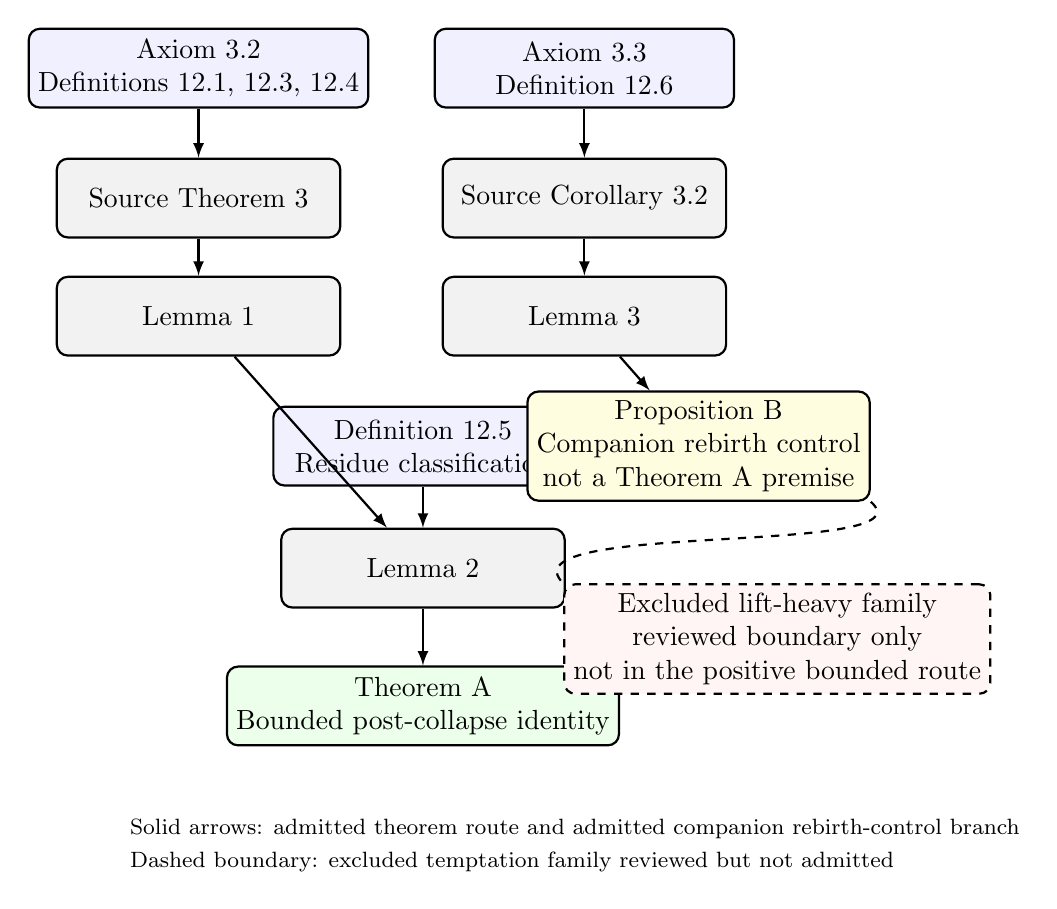
\begin{tikzpicture}[
    >=latex,
    thick,
    node distance=1.45cm and 0.8cm,
    proofnode/.style={draw, rounded corners, fill=gray!10, align=center, minimum width=3.6cm, minimum height=1.0cm},
    supportnode/.style={draw, rounded corners, fill=blue!6, align=center, minimum width=3.8cm, minimum height=1.0cm},
    excludednode/.style={draw, rounded corners, dashed, fill=red!4, align=center, minimum width=3.8cm, minimum height=1.0cm},
]

\node[supportnode] (leftsupport) at (0, 3.2) {Axiom 3.2\\Definitions 12.1, 12.3, 12.4};
\node[proofnode] (sourcethm) at (0, 1.55) {Source Theorem 3};
\node[proofnode] (lemmaone) at (0, 0.05) {Lemma 1};

\node[supportnode] (rightsupport) at (4.9, 3.2) {Axiom 3.3\\Definition 12.6};
\node[proofnode] (sourcecor) at (4.9, 1.55) {Source Corollary 3.2};
\node[proofnode] (lemmathree) at (4.9, 0.05) {Lemma 3};

\node[supportnode] (defresidue) at (2.85, -1.6) {Definition 12.5\\Residue classification};
\node[proofnode] (lemmatwo) at (2.85, -3.15) {Lemma 2};
\node[proofnode, fill=green!8, minimum width=4.1cm] (theorema) at (2.85, -4.9) {Theorem A\\Bounded post-collapse identity};

\node[proofnode, fill=yellow!12, minimum width=4.1cm] (propositionb) at (6.35, -1.6) {Proposition B\\Companion rebirth control\\not a Theorem A premise};
\node[excludednode] (excludedlift) at (7.35, -4.05) {Excluded lift-heavy family\\reviewed boundary only\\not in the positive bounded route};

\draw[->] (leftsupport) -- (sourcethm);
\draw[->] (sourcethm) -- (lemmaone);
\draw[->] (rightsupport) -- (sourcecor);
\draw[->] (sourcecor) -- (lemmathree);
\draw[->] (lemmaone) -- (lemmatwo);
\draw[->] (defresidue) -- (lemmatwo);
\draw[->] (lemmatwo) -- (theorema);
\draw[->] (lemmathree) -- (propositionb);

\draw[dashed] (propositionb.south east) .. controls +(0.8,-0.7) and +(-0.8,0.8) .. (excludedlift.north west);

\node[anchor=north west, align=left] at (-1.0, -6.2) {\footnotesize Solid arrows: admitted theorem route and admitted companion rebirth-control branch\\\footnotesize Dashed boundary: excluded temptation family reviewed but not admitted};

\end{tikzpicture}

\caption{Load-bearing theorem spine of the bounded Core~1.3 claim. The larger
monograph remains necessary because the surrounding chapters fix the ontology,
operator shell, K-level doctrine, collapse grammar, empirical bar, and audit
layers that keep this spine scientifically interpretable and externally
citable.}
\label{fig:oc13-theorem-spine}
\end{figure}

\subsection{What surrounds the spine}

The theorem spine is not self-sufficient. It is stabilized by the wider
manuscript in four distinct ways:

\begin{enumerate}
\item the formal doctrine chapters fix admissibility, thresholds, operators,
      levels, branching, and falsifiability;
\item the consistency and source-boundary chapters fix statement class,
      theorem fate, and publication scope;
\item the operational and empirical chapters fix promotion, replay, and
      falsifier discipline;
\item the appendices keep the audit and atlas burden inside the same volume.
\end{enumerate}

That is why the monograph is allowed to be larger than the defended article
without becoming rhetorically loose. The theorem spine is small; the lawful
scientific object surrounding it is not.

\subsection{Statement classes and burden}

\begin{table}[htbp]
\centering
\begingroup
\footnotesize
\RaggedRight
\setlength{\tabcolsep}{4pt}
\begin{tabular}{@{}L{0.21\textwidth}L{0.28\textwidth}L{0.39\textwidth}@{}}
\toprule
\textbf{Statement class} & \textbf{Scientific burden} & \textbf{Where to inspect it} \\
\midrule
Axiomatic statements & Fix primitive admissibility, identity, or threshold conditions. & Axiomatics, notation appendix, and Chapters~8--12. \\
Derived theorems and lemmas & Carry the proof-bearing positive body. & Results chapter, collapse and rebirth chapter, present roadmap, and reviewer appendix. \\
Structural statements & Explain hierarchy, module layout, and relation between levels or artifacts. & Chapters~10--15, 18, and 19. \\
Interpretive statements & Explain meaning, nonclaims, and downstream boundaries. & Discussion, worked examples, practical chapter, and the audit appendices. \\
Operational statements & Fix replay, comparator, falsifier, and escalation discipline. & Chapters~22--24 and Appendices~G--R. \\
\bottomrule
\end{tabular}
\endgroup
\caption{Statement classes and their inspection burden in Core~1.3. The table
does not replace the formal chapters; it simply prevents proof, interpretation,
and operational governance from quietly changing roles.}
\label{tab:oc13-statement-classes}
\end{table}

\subsection{Shortest hostile-review checklist}

If a reviewer wants the most efficient attack sequence, the logically hardest
checks remain the following:

\begin{enumerate}
\item verify that collapse is tied to loss of admissible realization rather
      than to loose metaphor;
\item verify that the irreversibility rule forbids restoration of the original
      continuum as numerically the same entity;
\item verify that residue and rebirth are controlled classifications rather
      than narrative labels;
\item verify that no excluded lift-heavy theorem family is smuggled back into
      the positive bounded route;
\item verify that the journal-core extraction says nothing stronger than the
      flagship monograph;
\item verify that the K-level doctrine, especially \(K_{11}\) and \(K_{12}\),
      is structurally justified rather than rhetorically inflated.
\end{enumerate}

If the release fails there, later prose cannot rescue it. If it survives
there, a slower full reading becomes worth the effort.

\paragraph{Bridge to the next chapter.}
With the proof route mapped, the next chapter changes mode deliberately. It no
longer navigates the spine abstractly; it shows how the formal grammar should
be read through worked examples, counterexamples, and bounded interpretive
checks.

\clearpage
